%%%%%%%%% SysML 2019 EXAMPLE LATEX SUBMISSION FILE %%%%%%%%%%%%%%%%%
%
%\documentclass{article}
%
%% Recommended, but optional, packages for figures and better typesetting:
%\usepackage{microtype}
%\usepackage{graphicx}
%%\usepackage{subfigure}
%%\usepackage{caption}
%\usepackage{subcaption}
%\usepackage{booktabs} % for professional tables
%\usepackage{microtype}
%\usepackage{graphicx}
%\usepackage[algo2e]{algorithm2e}
%\usepackage{booktabs} % for professional tables
%\usepackage{amsmath}
%\usepackage{amsfonts}
%\usepackage{minted}
%\usepackage{placeins}
%
%
%%\newcommand{\TODO}[1]{\textcolor{red}{TODO: {#1}}}
%%\newcommand{\TQC}[1]{\textcolor{red}{TQ: {#1}}}
%
%
%% hyperref makes hyperlinks in the resulting PDF.
%% If your build breaks (sometimes temporarily if a hyperlink spans a page)
%% please comment out the following usepackage line and replace
%% \usepackage{sysml2019} with \usepackage[nohyperref]{sysml2019} above.
%\usepackage{hyperref}
%
%% Attempt to make hyperref and algorithmic work together better:
%\newcommand{\theHalgorithm}{\arabic{algorithm}}
%
%% Use the following line for the initial blind version submitted for review:
%\usepackage{sysml2019}
%
%% If accepted, instead use the following line for the camera-ready submission:
%%\usepackage[accepted]{sysml2019}
%
%% The \sysmltitle you define below is probably too long as a header.
%% Therefore, a short form for the running title is supplied here:
%\sysmltitlerunning{The SeaNet Machine Learning Systems Optimization Environment}
%
%\begin{document}
%
%\twocolumn[
%\sysmltitle{The SeaNet Tensor Program Optimization Environment}

% It is OKAY to include author information, even for blind
% submissions: the style file will automatically remove it for you
% unless you've provided the [accepted] option to the sysml2019
% package.

% List of affiliations: The first argument should be a (short)
% identifier you will use later to specify author affiliations
% Academic affiliations should list Department, University, City, Region, Country
% Industry affiliations should list Company, City, Region, Country

% You can specify symbols, otherwise they are numbered in order.
% Ideally, you should not use this facility. Affiliations will be numbered
% in order of appearance and this is the preferred way.
%\sysmlsetsymbol{equal}{*}
%
%\begin{sysmlauthorlist}
%\sysmlauthor{Aeiau Zzzz}{equal,to}
%\sysmlauthor{Bauiu C.~Yyyy}{equal,to,goo}
%\sysmlauthor{Cieua Vvvvv}{goo}
%\sysmlauthor{Iaesut Saoeu}{ed}
%\sysmlauthor{Fiuea Rrrr}{to}
%\sysmlauthor{Tateu H.~Yasehe}{ed,to,goo}
%\sysmlauthor{Aaoeu Iasoh}{goo}
%\sysmlauthor{Buiui Eueu}{ed}
%\sysmlauthor{Aeuia Zzzz}{ed}
%\sysmlauthor{Bieea C.~Yyyy}{to,goo}
%\sysmlauthor{Teoau Xxxx}{ed}
%\sysmlauthor{Eee Pppp}{ed}
%\end{sysmlauthorlist}
%
%
%%EVALUATION TODOs (demo exploration)
%%Refactor SA Tuner to Proposer, Sampler, Cost Model
%%Search space stats (sizes for ARM CPU, CUDA GPU, x86 CPU, on ResNet-50, ResNet-18, VGG-19, MobileNetV2)
%%Peak Performance Comparison
%%Proposer Comparison (GA/"Evolutionary Algorithm", SA, Random)
%%Sampling Comparison (epsilon-greedy, k-means, random)
%%Cost Model Comparison (XGBoost, TreeRNN) (let's do fixed dataset), pick CUDA largest search space, x86 largest search space
%
%\sysmlaffiliation{to}{Department of Computation, University of Torontoland, Torontoland, Canada}
%\sysmlaffiliation{goo}{Googol ShallowMind, New London, Michigan, USA}
%\sysmlaffiliation{ed}{School of Computation, University of Edenborrow, Edenborrow, United Kingdom}
%
%\sysmlcorrespondingauthor{Cieua Vvvvv}{c.vvvvv@googol.com}
%\sysmlcorrespondingauthor{Eee Pppp}{ep@eden.co.uk}
%
%% You may provide any keywords that you
%% find helpful for describing your paper; these are used to populate
%% the "keywords" metadata in the PDF but will not be shown in the document
%\sysmlkeywords{Machine Learning, SysML}
%
%\vskip 0.3in
%
%\begin{abstract}
%Automatic machine learning program optimization is an exciting area for both systems and machine learning researchers, with significant progress being made at the kernel level of tensor programs---enabling powerful transformations.
%%For system researchers, this domain presents a new way to tackle traditionally difficult optimization problems that often required heavy manual intervention.
%%or machine learning researchers, the domain has the potential to be an exciting testbed for algorithmic ideas and innovation.
%%We are currently at an inflection point where significant progress in machine learning program optimization at the kernel level has the potential to enable more powerful transformations that span multiple levels of the stack and new operators in deep learning computation.
%However, rapid progress requires a common testbed to test and prove ideas. To this end, we propose both a common set of interfaces shared by many automatic kernel optimization strategies to improve the modularity of components required by different approaches and a dataset to help researchers efficiently prototype and evaluate ideas.
%Additionally, we design and implement an RPC system as the base of our optimization stack, which enables users to reuse their optimization pipelines and quickly collect data across a wide range of hardware devices.
%Finally, we evaluate a preliminary set of baseline optimization pipelines on different hardware devices to highlight the extensibility of the SeaNet environment.
%\end{abstract}
%]

% this must go after the closing bracket ] following \twocolumn[ ...

% This command actually creates the footnote in the first column
% listing the affiliations and the copyright notice.
% The command takes one argument, which is text to display at the start of the footnote.
% The \sysmlEqualContribution command is standard text for equal contribution.
% Remove it (just {}) if you do not need this facility.

%\printAffiliationsAndNotice{}  % leave blank if no need to mention equal contribution
%\printAffiliationsAndNotice{\sysmlEqualContribution} % otherwise use the standard text.

\section{Introduction}
%Many recent breakthroughs in machine learning have come from the ability to harness vast datasets and scale algorithms efficiently across various hardware devices and backends.
%This pattern is common across many domains e.g., XLNet in NLP, EfficientNet/AutoML for vision, and AlphaStar in reinforcement learning.
%Each advance has relied on scaling algorithms to previously intractable datasets and model sizes.
%Behind the scenes of each of these advancements is a scalable and efficient deep learning system; building performant systems for machine learning is a pressing research challenge.
%Automatic kernel optimization using machine learning has shown promise through preliminary results; well-designed search spaces can be automatically explored with machine learning algorithms to produce highly specialized implementations for machine learning kernels.
%These solutions demonstrate that these kernels are competitive with vendor-specific software libraries while requiring a fraction of the engineering effort, with the most gains being shown for esoteric or less popular workloads.
%However, even with many improvements to search time, current optimization algorithms require hours to days of search time for a model’s worth of kernels.
Machine learning program optimization is an important domain of research and the intersection of disciplines including computer architecture, deep learning, systems, and programming languages.
Most broadly, the goal of machine learning program optimization research is to enhance programmer productivity and hardware efficiency for research and production tasks.
Beyond program optimization, there has been tremendous progress in automatic optimization techniques to relieve the burden on human engineering effort at all levels of the hardware and software stacks.
Recent advances include automatic optimizations at the architecture~\cite{liu2018darts}~\cite{zoph2018learning}, graph~\cite{metaflow_sysml19}, kernel~\cite{NIPS2018_7599}, and hardware design levels~\cite{Koeplinger:2016:AGE:3007787.3001150}~\cite{koeplinger2018spatial}~\cite{moreau2019hardware}~\cite{8009208}, where performance is quickly becoming competitive with human engineers.
In work where the contribution requires human insight into model architectures (e.g., resolution and model width scaling~\cite{tan2019efficientnet} or novel combinations of \emph{operators} (e.g., convolutions with different kernel sizes) ~\cite{tan2019mixnet}, it is common to see the last mile of improvement being reached with automated methods such as neural architecture search (NAS).
However, in each subdomain of automatic optimization, there is room for standardized environments for evaluation.
In this paper, we focus on the rapidly developing line of work of kernel-level deep learning compilers~\cite{xing2019dnnvm}~\cite{222575}, where automated approaches show promise.

To advance the field, automatic program optimization must support a wide range of models: the commonplace, and the cutting edge across all deep learning domains.
However, automatic optimization research depends heavily on performance evaluation on real-world hardware.
Realistic benchmarks and systems for evaluation for researchers to perform high fidelity evaluations of proposed ideas and algorithms are crucial.
This raises a considerable barrier for researchers wishing to improve automatic optimization: compelling work must be general across many domains of models, yet also demon stably improve performance on real hardware and workloads.

Additionally, optimizing machine learning programs presents a broad and challenging problem domain with many reasonable choices for algorithms and modeling.
There has been little standardization of how to faithfully evaluate benchmarks or even which benchmarks are the most meaningful; the current trend has been to evaluate on a bag of popular models and report accuracy and performance numbers yet without any clear-cut method for others to extend (e.g., with new search techniques or algorithms) or \emph{reuse} existing work (e.g., on new models or new hardware devices).
%even when the pareto-optimality of such models and their fitness for a particular system or hardware backend is uncertain. %Examples of recent performance-driven evaluations, etc.
%This issue is exacerbated by the sheer height of the deep learning stack: every layer from hardware to model architectures presents optimization opportunities.

Furthermore, the rapid rate of innovation and daunting scope of cutting-edge machine learning models raises challenges for researchers aiming at building better systems.
At the core is the tension between innovation and replication: in order to perform a compelling evaluation of their work, researchers must typically replicate the entire end-to-end functionality of exiting deep learning software stacks.
This evaluation requirement comes at the cost of innovation as time must be dedicated to rebuilding portions of existing solutions rather than prototyping new ideas and system designs.
Consequently, performance-driven research and current deep learning breakthroughs are commonly months or years out-of-sync.
For example, depthwise convolutions were immediately adopted by the research community following the introduction of the MobileNet~\cite{DBLP:journals/corr/HowardZCKWWAA17} architecture---yet took considerable time to reach hardware specific vendor libraries. 
%Similarly, it is common to see computer architecture evaluations of hardware architectures that rely on models years from the state-of-the-art.
%TODO(reduce iteration time for hardware design)
%To reduce the burden on machine learning practitioners and researchers, we aim to standardize a benchmark environment to isolate machine learning challenges from s and infrastructure pain points, focusing on the realm of deep learning program optimization.

Finally, deep learning compiler research is a quickly moving subfield of systems research, with novel techniques being proposed at all levels of the stack, ranging from graph level transformations (e.g., operator fusion and more general graph rewriting)~\cite{metaflow_sysml19}~\cite{anderson2018optimal} and code generation (automatic kernel optimization) to semantic-altering transformations such as quantization~\cite{blott2018finn}~\cite{zhou2016dorefa}~\cite{fromm2018heterogeneous} and hardware-driven neural architecture search~\cite{Yang_2018_ECCV}.
%Current approaches are typically limited to exploring a constrained space of optimization techniques due to the sheer inherent difficulty of building a system capable of handling real-world models.
%For example, techniques may only consider a limited set of model operators, only leverage static performance models, or only be evaluated for a restricted set of hardware devices.
We aim to standardize a task for the sub-problem of optimizing deep learning programs at the granularity of single operators, or \emph{kernels}.


%To further complicate the scenario, researchers can be further siloed by the effort dedicated to building a sub-domain specific optimization system, as it is usually difficult to even attempt reproducing the evaluation of current work.
%In fact, the hardware platform(s) used in an evaluation have become a differentiating factor for performance-driven research.
%Along these lines, we have seen the bifurcation of "efficient" model architectures into multiple domains: the MobileNet(s) (e.g., MNASNet), which make heavy use of "mobile-friendly" depthwise convolutions, and more expensive architectures (e.g., NASNet, AmoebaNet), which leverage full convolutions.
%Even within "mobile" oriented deep learning research, there are several opportunities for improvement via a benchmark framework that supports a diverse set of hardware backends.
%A prevailing argument in favor of depthwise convolutions and their use in "mobile-oriented" scenarios are their reduced arithmetic intensity that are more suited to CPU architectures.
%However, this argument makes the assumption that mobile CPUs are comparably more efficient than their GPU counterparts.
%Additionally, if such reduced arithmetic intensity is a valuable asset for CPU architectures, it would also make sense to perform serious evaluation of depthwise convolution-backed networks on server CPU architectures, which are likely to be a key component in datacenter inference systems.

% modifications to existing framework compilation (ad-hoc, composable)? 
% supported collection of models 
% no guarantees

% not portable across hardware devices

% to the point that similar approaches are considered novel based on their evaluation settings ???


%One issue is that research in this area often focuses on a local aspect of compilation (e.g., graph rewriting), with the implicit assumption or hope that all other aspects are orthogonal.
%For example, optimizations such as operator fusion and neural architecture search are often driven by heuristics or the implicit assumption that all operator costs are static or known ahead of time.
%Even as this implicit assumption is invalid, 


%While this iteration time can be acceptable for inference-heavy workloads, it is not acceptable for training workloads where the operator tuning time could be allocated to model training instead. Long tuning time also precludes running operator optimization in the inner loop of higher level optimization algorithms, such as (relaxed graph substitutions, operator fusion proposal, your compiler pass here).
%This limitation has meant that current graph-level optimization work must rely on fixed software libraries with limited potential for generating new variants of operators, biasing results towards kernels with the most dedicated engineering time.
%For example, even "proxyless" approaches are typically reliant on a hardware vendor-specific pre-tuned library for performant kernel implementations.
%While hardware vendors are strongly incentivized to provide high performance implementations of popular deep learning worklods, they are constrained by engineering resources, biasing performance towards the most widely-used model architectures.
%In turn, this limits the optimization scope of performance-driven deep learning research.


%Additionally, the lack of common optimization benchmarks means that improvements to a given task or hardware are seldom ported to other, highly similar problem domains.
%For example, the difficulty in performance-driven optimization techniques (e.g., neural architecture search) to different hardware platforms has meant that prior work (e.g., MNASNet, ProxylessNAS) is usually restricted to single-target evaluations.
%We see the issue as fundamentally being one of brittle or cumbersome support for hardware devices and deep learning operators.
Researchers stick with known workflows with short evaluation times: defining and optimizing operators for a new hardware device takes time.
Alternatively, efficient and flexible code-generation for hardware devices dramatically reduces the iteration time for hardware architects and adoption burden for end-users.
Performance-driven deep learning researchers have noticed this limitation~\cite{barham2019machine}.
Projects such as TensorFlow XLA and NVIDIA TensorRT are scrambling to cover and support as many workloads demanded by researchers and practitioners as possible, and automated techniques are attractive for such tasks, yielding ripe research opportunities.
%However, we currently lack a cohesive and standardized environment to evaluate optimization approaches.
%In addition to questions such as: what algorithm is best for searching my discrete space of optimizations, we lack answers to more basic questions such as the typical workload mix of researchers and practitioners.

The central issue is the absence of a unified \emph{environment} and \emph{dataset} for machine learning program optimization that allows researchers to quickly prototype algorithms in a device-agnostic fashion.
%TODO: first pass is currently aiming to get the text down
%ideally, we want to distill these into a few central points, and potentially refactor into a different section other than Motivation/Background?
We introduce the SeaNet to provide an easily extensible automatic deep learning program optimization environment, with datasets provided to allow researchers to quickly explore ideas and algorithms.
%Deep learning research has seen tremendous success with emerging model architectures (e.g., EfficientNet, ProxylessNAS) and operators (e.g., Depthwise convolution, Attention).
%At present, the design of architectures and operators is often constrained to variations of kernels that are implemented in current vendor-specific libraries.
%For example, Attention relies on matrix multiplication as its core primitive, and current vision models such as EfficientNet do not stray from typical vision operator shapes (e.g., 3$\times$3 convolution).
%In order for deep learning research to be uncurbed by software limitations, performant kernels should be generated for arbitrary operator definitions and hardware platforms.
\begin{figure}[ht]
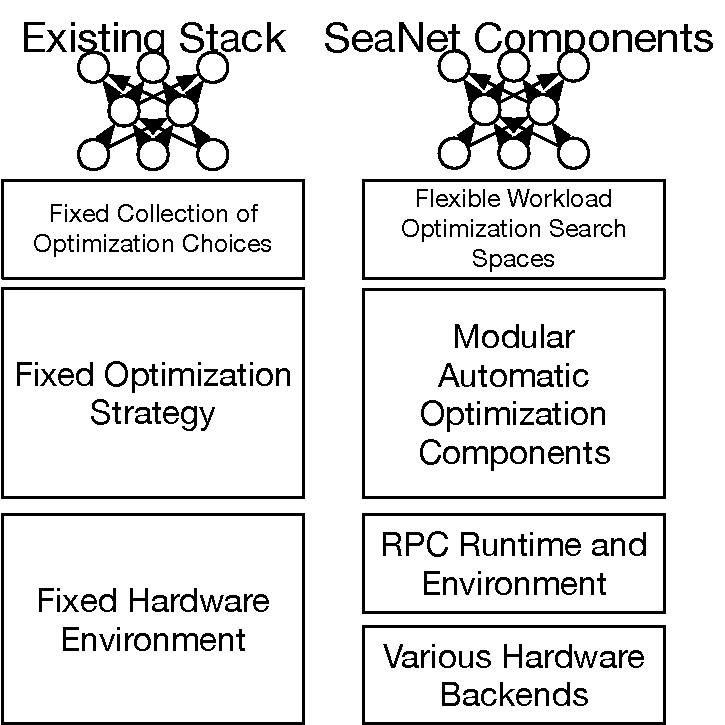
\includegraphics[width=\textwidth]{sys_diagrams/overview2.pdf}
\caption{SeaNet provides flexibility and extensibility to existing deep learning program optimization stacks.
Researchers can use SeaNet to experiment with novel automatic optimization components for off-the-self of bespoke models. Hardware engineers and researchers can propose new search spaces of optimizations for deep learning operators. SeaNet can be used to build collections of optimized kernels for low level system libraries (e.g., cuDNN, MIOpen).}
\end{figure}


The contributions of this paper are as follows:
\begin{itemize}
\setlength\itemsep{0em}
\item We introduce the SeaNet automatic optimization environment.
\item Alongside several reference benchmark tasks for machine learning program optimization, we introduce an API for researchers to plug in custom algorithm implementations.
\item We provide a cross-platform RPC runtime-system that supports a wide range of hardware devices.
\item We include baselines for each of our benchmark tasks.
\end{itemize}
%We are inspired by the impact of (x y z ImageNet, DawnBench) benchmarks in other areas in terms of improvements towards on an important and shared goal of the community.
%Traditionally, dramatic breakthroughs in research domains have been preceded by new datasets that enabled the efficient exploration and scaling of novel ideas (e.g., ImageNet for vision, GLUE for NLP).
%Standardization gives researchers confidence that their comparisons are valid and their results reproducible and the opportunity for the rapid extension and iteration of existing solutions.
%Perhaps most importantly, it eliminates the burden of collecting vast datasets just to test a proof-of-concept or reach parity with other researchers.

%To address these challenges, we define the NAME automatic optimization benchmark and environment.
%In addition to defining a set of concrete optimization tasks, NAME includes critical infrastructure to aid researchers in bootstrapping the evaluation of their solutions. The NAME infrastructure includes: a distributed RPC system to scale tasks across a diverse collection of hardware devices, a common optimization API to target to facilitate modular implementations, and a collection of reference datasets to quickly prototype ideas.
%Finally, we provide a set of reference implementations to be used as strong baselines.

%\section{Related Work}
%SeaNet presents an environment for deep learning kernel optimization; this environment can be analogous to simulation environments for reinforcement learning agents, where researchers can prototype ideas and algorithms without needing to build a virtual or physical world from scratch.
%Ray~\cite{222605} is an analogous environment for reinforcement learning.
%SeaNet differs in its performance-driven objective that can leverage measurements on real hardware and the ready availability of out-of-the-box benchmarks (e.g., reference workloads such as popular computer vision models).
%Park~\cite{mao2019park} is an environment for reinforcement learning-based optimization for general systems challenges, such as device placement, circuit design, and load balancing.
%While reinforcement learning can also be applied to the challenge of automatic kernel optimization, we focus on providing generic support for optimization pipelines for a wide breadth of hardware devices and kernels.
%Similarly, Vizier~\cite{golovin2017google} presents an optimization service for general blackbox functions.
%The SeaNet environment can be viewed as a Vizier-like service for whitebox deep learning kernels where support for experimenting with the optimization algorithms themselves is a design goal.
%
%
%On the benchmark front, SeaNet is analogous to recent work such as NAS-Bench-101~\cite{pmlr-v97-ying19a} which provides a reference dataset for NAS alongside benchmark tasks.
%However, we while we provide a dataset, we do not settle on a fixed dataset as hardware targets and models are continuously evolving.
%SeaNet benchmark tasks have a similar flavor to the NAS-Bench tasks, as neural architecture search presents a discrete optimization problem similar in structure to that of program optimization.
%Concretely, the main differences are in the feasibility of evaluation (seconds vs. hours to evaluate candidates), and the objectives (performance vs. validation accuracy).
%Additionally, we encourage SeaNet users to collect performance data and run experiments on hardware that they have available, whereas this may not be feasible for NAS-Bench tasks.
%However, it is entirely possible that variations of successful kernel optimization algorithms and pipelines can be successfully applied to neural architecture search, and we hope to see cross-pollination across the problems.
%
%
%The task of automatic program optimization is not new, and has been recently visited with several different approaches, such as analytical models~\cite{mullapudi2016automatically}, statistical cost model guided search~\cite{NIPS2018_7599}, tree search~\cite{Adams2019LearningTO}, static cost models~\cite{Kim:2019:CGH:3314872.3314885}, and statistical cost models driven by handpicked features~\cite{Li:2018:DPI}.
%SeaNet aims to provide a flexible framework for researchers to explore new innovations.
%%Differences (performance driven), and measurements also happen on real hardware (are feasible) vs. difficulty of deploying agents to real environments.
%%SeaNet presents both an \emph{environment} for automatic optimization experiments, and a \emph{dataset} for prototyping.
%Additionally, parallel work on machine learning for systems work includes automatic device placement~\cite{mirhoseini2017device}, graph optimization~\cite{metaflow_sysml19}, parallelization~\cite{soap_sysml19}, architecture search~\cite{tan2019mnasnet}~\cite{zoph2018learning}, among others. 

\section{SeaNet Workflows and Tasks}
\label{sec:tasks}
We describe the typical tasks we aim to optimize via SeaNet in this section.
Posed as questions, they can be described as: \textbf{(1) How can I quickly generate the best code (optimization) for the operators in a deep learning model?} \textbf{(2) How can I predict the peak-performance of a given workload?}
Here, workload refers to a deep learning \emph{operator} (e.g., convolution, matrix multiply, or attention) with some instantiated \emph{shape} (e.g., kernel sizes, input sizes, or strides). 
Concretely, an instance of the first task could be: ``optimize all convolution and matrix multiply shapes found in a model such as ResNet-18."
Similarly, an instance of the second task could be: ``what is the predicted latency of all the convolution and matrix multiply shapes in InceptionV3?"


The first question arises from the challenge of deploying a model to a hardware target.
In this setting, a researcher or developer has prepared a deep learning model for some application, and wishes to compile the optimal version for some target hardware (e.g., cloud servers, mobile phones, IoT devices, etc.).
%We frame this task in a framework of combinatorial optimization.
Given a single workload out of a collection of workloads presented in a model, generating the optimal code can be approximated by choosing the right configuration for a set of choices in a discrete search space.
We describe the search space in more detail in~\autoref{sec:rpc}.
These knobs can be attributes such as the tiling of loops in the workload, the parallelization strategy, memory layout, etc.
We expect this task to be driven by statistical methods that rely on \emph{measurements on real hardware} or \emph{simulation} in the optimization loop, as shown in~\autoref{fig:overview}.
Accordingly, the \emph{cost-modeling} aspect of this task can be modularized and evaluated in isolation using a static dataset, which we provide alongside SeaNet.


The second question arises from the challenge of performance driven neural architecture search.
This challenge is an emerging task, with particular relevance in latency-driven settings (e.g., mobile inference workloads)~\cite{tan2019mnasnet}~\cite{2018arXiv181200332C}.
Whereas classical neural architecture search focuses on the singular objective of optimizing accuracy or loss on some validation set, performance driven neural architecture search aims to balance accuracy with some hardware constraint, such as \emph{latency}.
Unfortunately, when the performance of each architectural choice (usually at the granularity of workloads) is no longer easily obtainable via a static library, performance-driven optimization becomes infeasible without rapid performance estimates from another source.

To address this issue, we introduce the task of \emph{peak-performance prediction}.
Peak performance prediction takes as input a collection of pre-optimized workloads (e.g., workloads that have already been optimized in accordance with the first task), and the corresponding performance achieved on each workload after tuning.
The objective is to accurately predict the performance of a previously \emph{unseen} workload, so that an outer algorithm such as neural architecture search can decide if the workload is worth using or optimizing.
Additionally, peak performance prediction is useful even when the collection of fixed workloads to be optimized is fixed: an optimization system can use peak performance prediction to prioritize optimization resources between the different workloads, as workloads that are already at their predicted maximum performance can be deprioritized.

\section{SeaNet Developer API}
In this section, we present a the SeaNet modular automatic optimization pipeline aimed at tackling the first task of generating the best operator implementations using as few evaluations of a simulator or real hardware as possible.
The pipeline starts from a \emph{search space} of possible implementations for each program, with up to billions of \emph{configurations} (a point in the search space with instantiated values for all tunable implementation parameters).
Next in the pipeline is \emph{model optimizer}, which proposes promising configurations to a \emph{cost-model} or value function, which estimates the performance of the proposed configurations.
These performance results are filtered by a \emph{sampler} that  decides which configurations to evaluate on real hardware. This pipeline is shown with a concrete example in~\autoref{fig:overview}.
After a round of measurements on hardware, the cost model is updated and the pipeline repeated.
One critical feature of the optimization API is that it is device-agnostic, as simulator and performance measurement on hardware devices is handled by the RPC subsystem (\autoref{sec:rpc}) of SeaNet.
%Previous works (?? NAS, Proxyless) have shown that considering the performance implications of optimizing deep learning computation (e.g., through NAS) can yield appreciable real-world gains.


\begin{figure}[tb]
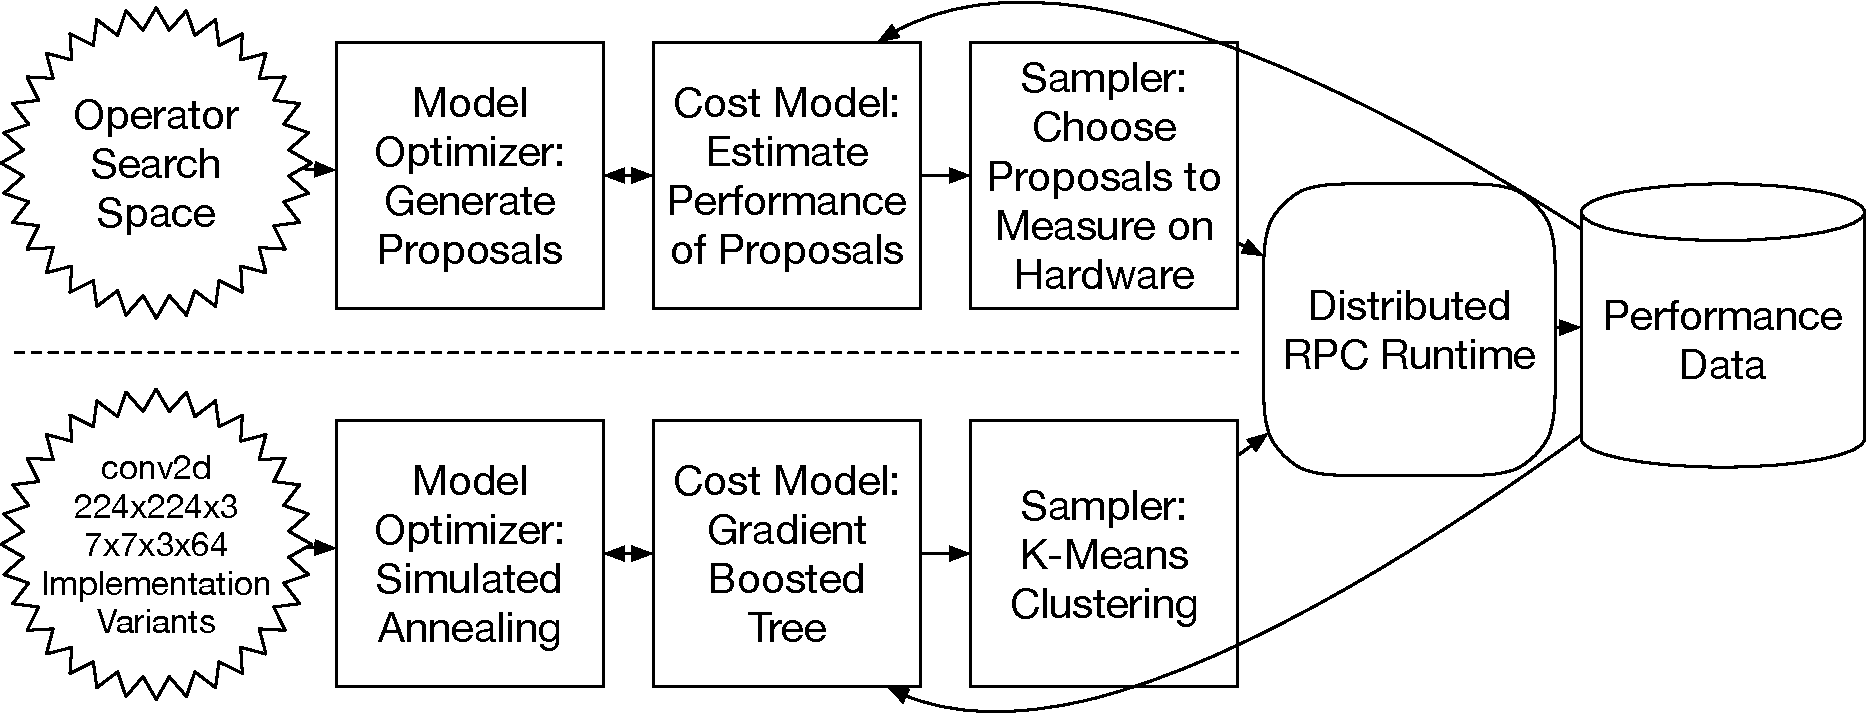
\includegraphics[width=\textwidth]{sys_diagrams/plug.pdf}
\caption{
Organization of optimization modules outlined by the SeaNet benchmark task: the proposer (model optimizer), cost model, and sampler. The bottom half denotes an example pipeline instantiated with concrete options for each of the modules.}
\label{fig:overview}
\end{figure}
%We describe several concrete experiment flows in this section.
%The original AutoTVM work has seen success in specialized systems projects; we wish to extend the ability to do such work to the broader machine learning community.
%We outline several components that can be used to compose an optimization pipeline in this section: comparing the performance of cost models, sampling strategies, and proposal methods.
%For the first task, the system takes as input a search space of deep learning operator configurations and an associated hardware target for deployment.
%While the search space is discrete, it is composed of many interrelated parameters which each present a collection of choices.
%Typically, current solutions rely on machine learning based cost models to guide the search process, meaning that time is used both on optimization algorithm and data collection (measuring the performance of configurations on real hardware).
%As both sides contribute to the wall-clock time used by the %solution, the system must balance available (compute) resources for machine learning algorithms and the hardware target effectively.
%*note on balance of system resources, e.g., hardware for cost model evaluation, and hardware for measurement*

%We identify several system components shared by many classes of solutions. Optimizing any single component will improve the performance of the optimization system, though the impact of improvement will depend on the current balance of system resources.
%These components include a \emph{model optimizer}, which proposes promising configurations to evaluate (either with a cost model or on real hardware), a cost model (which provides an estimation of the performance of a configuration without relying on real hardware, and a sampler (which takes a batch of proposed/evaluated configurations and decides which to use for real data). We provide more detailed descriptions of each with examples below.
Each of these modular components can be implemented with algorithms of varying complexity.
For example, a model optimizer could simply propose random configurations, use heuristics such as simulated annealing, or contain a machine learning model itself (e.g., in the case of a reinforcement learning agent).
Similarly, a cost model may be a gradient tree-boosting model taking in AST-level features as input, or a TreeGRU~\cite{Tai2015ImprovedSR} model operating on program ASTs directly.
Sampling algorithms range from greedy samplers (measure the top-$k$ most promising configurations according to the cost model), or more disciplined techniques that attempt to balance exploration and exploitation (e.g., using $k$-means~\cite{DBLP:journals/corr/abs-1905-12799} clustering to blend similar data points together).
Finally, a researcher may choose to eschew implementing some or all of the modules in favor of alternative strategies, such as a RL-agent based method.
In such a strategy, the model optimizer simply becomes a wrapper around an RL algorithm and the sampler becomes a passthrough.

%These uses cases arise from a typical optimization pipeline, where a user has a fixed inference graph to be optimized for some target hardware device.
%We assume that the optimal choices of kernel variations (which algorithm to use for each operator in the model) have already been made (or that we must exhaustively optimize all of them).
%In this setting, the objective is to find the fastest implementation of each kernel by choosing the best setting for a collection of tuning knobs in the shortest total wall-clock time.
%Each kernel has a discrete optimization search space defined by the knobs contained in its \emph{schedule template}.
%We provide an example of a kernel and its associated schedule template in fig??.
%A variation of this setting is to prioritize each kernel such that the end-to-end network time is at its lowest at any possible stage of optimization---we omit this for now.

\subsection{Model Optimizer API}
As it is often too expensive to exhaustively estimate the performance of all possible configurations of a  kernel, an efficient \emph{model optimizer} is crucial in deciding promising candidates.
Blackbox proposal strategies include genetic algorithms, random search, and many Bayesian optimization strategies.
Similarly, if we consider each configuration to exist in a connected discrete search space, we can view the task as a traversal problem applicable to reinforcement learning and simulated annealing.
Here, the objective is to propose the most performance kernel configuration given as few cost model or real-hardware evaluations as possible.
For blackbox models, this amounts to the fewest number of iterations---and for the statistical approaches, this amounts to the fewest training examples.

The model optimizers are queried for updated \emph{proposals} or promising configurations to evaluate on real hardware.
To implement a model optimizer, the user needs only to implement a single function in the interface, \texttt{find\_maximums}, which is called to collect a batch of proposals.
Intuitively, the \texttt{find\_maximums} is called to get configurations that maximize the performance returned by the cost model.
We show an example of a model optimizer in listing ~\autoref{lst:modeloptimizer}.
%
%\begin{listing}[ht]
%\begin{minted}
%[
%frame=lines,
%framesep=2mm,
%baselinestretch=1.2,
%%bgcolor=LightGray,
%fontsize=\footnotesize,
%linenos
%]
%{python}
\begin{lstlisting}[caption={Simple example of a naive random model optimizer. A reference to a cost model is passed as \emph{model}, the number of proposals is specified with \emph{num}, and \emph{excl} contains a set of any points in the search space that should be excluded from consideration.},label={lst:modeloptimizer},language=Python]
def find_maximums(self, model, num, excl):
    self.visited = set()
    size = len(self.task.config_space)
    for i in range(0, n_iter):
        roll = np.random.randint(0, size)
        if roll in self.visited or\
           roll in excl:
            continue
        else:
            self.visited.add(roll)
            rolls += roll 
    picked = rolls
    for i in range(0, self.n_iter):
        self.visited.add(rolls[i])
    scores = model.predict(picked)
    points = sorted(picked, key=lambda item: 
        scores[picked.index(item)],
    reverse=True)
    return points[:num]
\end{lstlisting}

%\end{minted}
\subsection{Cost Model API}
While evaluating the performance of proposed kernels is relatively cheap compared to traditional Bayesian optimization settings, hardware resources typically limit the number of feasible experiments (kernels to profile on real hardware) to the order of thousands for practical problems.
This limitation means that cost models (either statistical, analytical, or simulated) are often useful for boosting the performance of algorithms that rely on some estimate of performance.
One subproblem of optimization can be viewed as building an accurate and efficient cost model---one that faithfully captures the performance of hardware with relatively few samples.
Ideally, such a cost-model should also be generalizable across hardware devices to avoid the engineering burden of specializing cost-models for each and every target hardware platform.

A cost model implements a minimum of two functions: \texttt{fit}, and \texttt{predict}.
\texttt{fit} takes as input a set of data points (configurations and their corresponding perfomance) in a canonical format, and updates the state of the cost model given the new data.
\texttt{predict} takes as input a set of configuration points, and outputs their corresponding costs.
We show a sample implementation of a cost model in listing ~\autoref{lst:costmodel}.

%\begin{listing}[ht]
%\begin{minted}
%[
%frame=lines,
%framesep=2mm,
%baselinestretch=1.2,
%%bgcolor=LightGray,
%fontsize=\footnotesize,
%linenos
%]
%{python}
\begin{lstlisting}[caption={Simplified example of a gradient tree boosting cost model using the XGBoost~\cite{chen2016xgboost} library. \texttt{\_get\_feature} can be any function that presents an arbitrary feature representation to the cost model. For example, this representation may simply be a concatenation of the choices, an AST representation of the lowered code, or a dataflow graph of operations.}, label={lst:costmodel}, language=Python]
def fit(self, xs, ys,...):
    x_train = self._get_feature(xs)
    y_train = np.array(ys)
    y_max = np.max(y_train)
    y_train = y_train / max(y_max, 1e-8)
    index = np.random.permutation(len(x_train))
    dtrain = xgb.DMatrix(x_train[index],
                         y_train[index])
    self._sample_size = len(x_train)
    self.bst = xgb.train(...)
def predict(self, xs,...):
    feas = self._get_feature(xs)
    dtest = xgb.DMatrix(feas)
    return self.bst.predict(dtest)
\end{lstlisting}
%\end{minted}


\subsection{Sampler API}
Additionally, reducing the number of proposed configurations to a feasible number that are measured on real hardware is an effective way to speed up the optimization loop.
One observation is that implementation search spaces can contain many configurations or programs that are close both in terms of performance and in terms of configuration.
Identifying this scenario and pruning configurations that are likely to be similar reduces the amount of hardware time needed to train an accurate cost model or find performant examples~\cite{DBLP:journals/corr/abs-1905-12799}
A sampler takes in a collection of configuration proposals and chooses $k$ proposals to be evaluated (e.g., on real hardware or in simulation).
A sampler only needs to implement a \texttt{sample} function, which takes the proposals, their corresponding costs (as evaluated by the cost model), and $k$ as input.
We show an example of a sampler in listing ~\autoref{lst:sampler}.

%\begin{listing}[ht]
%\begin{minted}
%[
%frame=lines,
%framesep=2mm,
%baselinestretch=1.2,
%%bgcolor=LightGray,
%fontsize=\footnotesize,
%linenos
%]
%{python}
\begin{lstlisting}[caption={Example of a $k$-means clustering based sampler that attempts to achieve sample diversity. Points refers to the current proposed set of configurations, scores are their corresponding scores as given by a cost model, and the plan size is the number of points (configurations) that should be selected for measurement.},label={lst:sampler},language=Python]
def sample(self, points, scores, plan_size):
    #convert configuration index to coordinates
    X = [point2knob(point, self.dims)
         for point in points]
    kmeans = cluster.KMeans(plan_size)
    means = kmeans.fit(X).cluster_centers_
    means = np.round(means)
    plan = [int(knob2point(mean, self.dims))
            for mean in means]
    return plan
\end{lstlisting}
%\end{minted}
%We show evaluations of baseline proposer-cost-model-sampler pipelines in the results section.



%For the first task, the general organization of the SeaNet API follows an object-oriented style.
%Developers and researchers may optionally override base classes for the \emph{model optimizer}, \emph{cost model}, and \emph{sampler} to implement bespoke solutions to the optimization task.
%
%An issue present in many current implementations, however, is that they are usually specialized for a single hardware target even when the algorithm itself may generalize well to other hardware targets and deep learning workloads.
%For the second task of peak-performance prediction, a canonical data format is sufficient as it maps well to any machine learning approach capable of performing regression.

%\section{SeaNet as a Benchmark}
%We introduce concrete benchmarks in this section that correspond to typical optimization tasks.
%As a representative example, we include benchmarks for the efficiency of optimization algorithms when searching for the best operator implementation.
%Here, we focus on convolution operators popular in deep learning models across a range of hardware devices.
%The objective is to find an implementation that yields the shortest execution time with as few invocations of real hardware as possible.

\section{SeaNet as a Dataset}
We provide a dataset to quickly evaluate deep learning kernels out of the box in two ways:  per-configuration performance for a fixed search space, and peak prediction performance for a given workload (e.g., Conv2D with a certain shape).
Users can use data for the first scenario to prototype cost models for Task 1 (introduced alongside Task 2 in ~\autoref{sec:tasks}), and data for the Task 2 scenario to prototype peak performance prediction models.
Additionally, users are free to collect their own dataset using in-house hardware devices by leveraging SeaNet's search space definitions for deep learning operators.



\subsection{The Configuration Search Space}
\label{sec:searchspace}
\begin{figure}[tb]
    \centering
    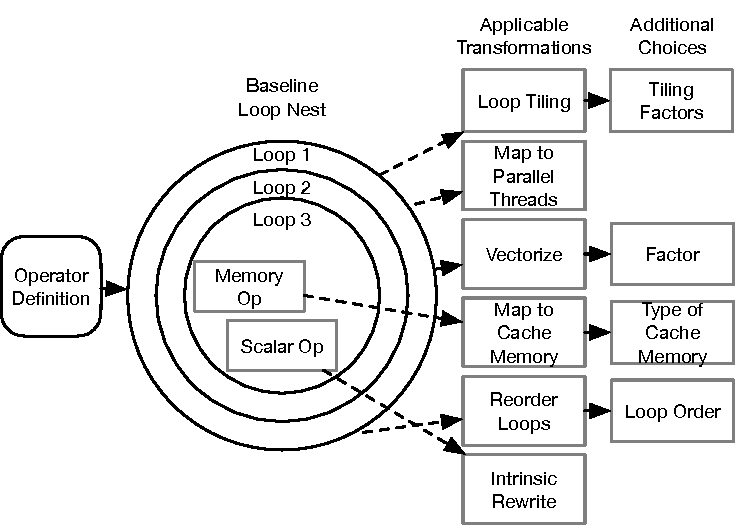
\includegraphics[width=\textwidth]{sys_diagrams/searchspace.pdf}
    \caption{Organization of an operator search space in SeaNet following its operator definition. Deep learning kernels present a loop nest of operations, with various transformations available to different components of the loop nest. Depending on the transformation, additional parameters may need to be decided. Note that the search space definition can be recursive (e.g., if a loop nest is tiled, the resulting loop nest can optionally be further tiled).}
    \label{fig:searchspace}
\end{figure}
The SeaNet API gives access to a rich collection of kernel implementation search spaces for common deep learning models on a wide range of hardware backends, ranging from ARM and x86 CPUs to mobile OpenCL GPUs and CUDA server-class GPUs.
~\autoref{fig:searchspace} gives a logical overview of an example search space.
This search space is built on top of \emph{schedule primitives}~\cite{ragan2017halide}~\cite{222575} that describe possible optimizations to apply to kernels.
These search spaces define possible implementations of deep learning kernels for their corresponding hardware devices.
The complexity of a search space varies depending on the target hardware device and operator, with the largest search spaces comprising billions of configurations.
Typically, we find that search spaces for devices with intricate memory hierarchies (e..g, GPUs) have more configurations (to cover the wide variety of program implementations) and are more difficult to optimize due to the sharp performance cliffs associated with cache hierarchies.


\subsection{Standalone Configuration Performance Prediction}
We provide several sample datasets spanning thousands of configuration points for rapid prototyping of cost models.
These datasets are obtained from randomly sampling the optimization search space of a typical convolution operator (e.g., from a ResNet model) on various hardware devices.
These datasets are collected from a range of hardware devices (desktop GPU, mobile CPU, and mobile CPU) and cover a wide range of performance.
Concretely, the dataset is a collection of configurations (possible implementations of a given workload), to their measured performance on hardware.
~\autoref{tbl:costmodelbaseline} shows a comparison of baseline cost models on this dataset.
Note that a SeaNet user can quickly collect a comparable dataset on other hardware devices they have available by leveraging the RPC infrastructure (~\autoref{sec:rpc}).
Data collection is fast, usually on the order of thousands of configuration points per hour.
\begin{table}[]
    \centering
    \begin{tabular}{l|c}
    \hline
    \multicolumn{2}{c}{1080 Ti (Desktop GPU)} \\
    \hline
    Cost Model&MAE (GFLOPS)\\
    \hline
    Linear Regression & 52.6 \\
    2-MLP & 49.6  \\
    Gradient Tree Boosting &  \textbf{44.7}\\
    \end{tabular}
        \begin{tabular}{l|c}
    \hline
    \multicolumn{2}{c}{ARM Cortex A-72 (Mobile CPU)} \\
    \hline
    Cost Model&MAE (GFLOPS)\\
    \hline
    Linear Regression & 1.40 \\
    2-MLP & \textbf{1.23} \\
    Gradient Tree Boosting & 1.34\\
    \end{tabular}
    \begin{tabular}{l|c}
    \hline
    \multicolumn{2}{c}{Mali T-860 MP4 (Mobile GPU)} \\
    \hline
    Cost Model&MAE (GFLOPS)\\
    \hline
    Linear Regression & 3.09 \\
    2-MLP & 3.77 \\
    Gradient Tree Boosting & \textbf{1.69}\\
    \end{tabular}
    \caption{Standalone evaluation of various cost model baselines on workloads collected from different hardware devices.
    MAE refers to the mean absolute error of the regression on a held-out set in billions of floating-point operations per second. Note that the absolute scale difference can be partially attributed to the typical peak performance achievable on each hardware device.}
    \label{tbl:costmodelbaseline}
\end{table}


\subsection{Peak Performance Prediction}
\label{sec:peakperformance}
Additionally, we provide a dataset of pretuned operators for thousands of workloads found in popular deep learning models, corresponding to thousands of hours of machine time.
These pretuned operators correspond to specific configurations expected to approximate the peak performance of a given hardware device for these workloads.
Predicting peak performance is an important task for areas such as graph optimization and performance driven neural architecture search.
In this setting, a model is trained on data that maps a collection of pretuned workloads (based on features such as their shapes, implementation strategy, and the hardware type) to achieved performance.
An accurate model is critical when optimization is too expensive to run in the loop of a larger NAS or graph optimization pipeline.
Concretely, the peak prediction dataset can be viewed as a mapping of workloads (a given operator with specific semantics such as shape, stride, padding) to latency (execution time).
%Such a dataset allows for peak-performance prediction experiments.
%Additionally, form of prediction is important for two subtasks in automatic optimization: prioritization, and graph optimization.


%We provide summary statistics of the peak performance dataset in \TODO{??}.
\section{Distributed RPC Infrastructure}
\label{sec:rpc}
All of the data collected for the tasks discussed thus far and the environment depends on the SeaNet RPC infrastructure.
This section discusses the low-level infrastructure used to collect performance measurements (either for building or a dataset, or in an online experiment) from hardware.
Deep learning compiler optimizations are typically highly specialized to leverage domain-specific insights about their workloads.
%However, the compiler techniques themselves should be general, as the ubiquitous nature of deep learning tasks means that they are deployed to a wide variety of hardware targets.
As evaluating compiler optimizations on multiple hardware and software platforms quickly becomes tedious, we provide a generic RPC Infrastructure as part of the SeaNet environment.
Crucially, this infrastructure is \emph{transparent} to the researchers developing new optimization algorithms.
%Only when new classes of hardware devices are added are extensions to the RPC infrastructure required.
%The RPC infrastructure allows researchers to scale their experiments across many different hardware devices, but also to develop solutions that are agnostic to any target hardware platform or runtime.
%The most basic use-case of the RPC system is to measure the performance of some compiled code---the functionality on which the rest of the system relies.
Under the hood, the RPC system also provides tremendous flexibility as it enables fine-grained control of the device runtime.
For example, the RPC system enables us to ensure that idiosyncratic system parameters (e.g., CPU affinity on a big.LITTLE SoC) are correctly configured.

%\subsection{Addressing Threats to Reproducibility}
One of the main advantages of having a shared framework for benchmarking optimization algorithms is reproducibility.
Modern machine learning pipelines commonly have numerous hyperparameters and subtle implementations differences that often go unreported in published work yet can make profound differences in evaluations results.
Due to the systems-performance driven nature of kernel optimization, hyperparameters now threaten reproducibility on two frontiers: experiment configuration and measurement.
In addition to experiment hyperparameters, the conditions of performance measurement (e.g., how wall clock execution time is measured) is often an ad-hoc choice left to researchers. Conveniently, sharing a common RPC infrastructure for evaluating optimization algorithms allows the burden of sensible performance measurement guidelines to be collectively addressed: wisdom about the idiosyncrasies of each hardware platform can be shared instead of being independently discovered through each evaluation.
Examples of pitfalls that researchers must account for/discover include: JIT kernel compile time (for languages such as CUDA and OpenCL), hardware power states that take time to warm-up/cool down (virtually all modern CPUs and hardware accelerators), and thermal throttling on devices with limited thermal dissipation (e.g., single-board computers and mobile phones).
We provide customized RPC \emph{servers} for a variety of hardware platforms to alleviate the burden of device-specific housekeeping on researchers.
%Just as importantly, a shared framework allows the community to collectively agree on a set of reasonable protocols and procedures and measurements.

%\subsection{RPC System Overview}


\subsection{RPC Protocol}
At a high level, the RPC system is composed of a central tracker which multiplexes RPC servers across many RPC sessions.
RPC servers can be individual mobile phones, single-board computers (e.g., Raspberry Pi, RK33999), hardware accelerator boards (e.g., Ultra96), or servers hosting multiple GPUs and CPUs.
%Each time 
We describe our RPC protocol in two parts: a \emph{control} plane which handles resource allocation and load balancing across many hardware devices, and a \emph{data} plane which handles communications between hardware devices and clients issuing requests.
Together, these components of the protocol enable streamlined prototyping and deployment of neural network implementations.
\paragraph{Control Plane}
\begin{figure}[t!]
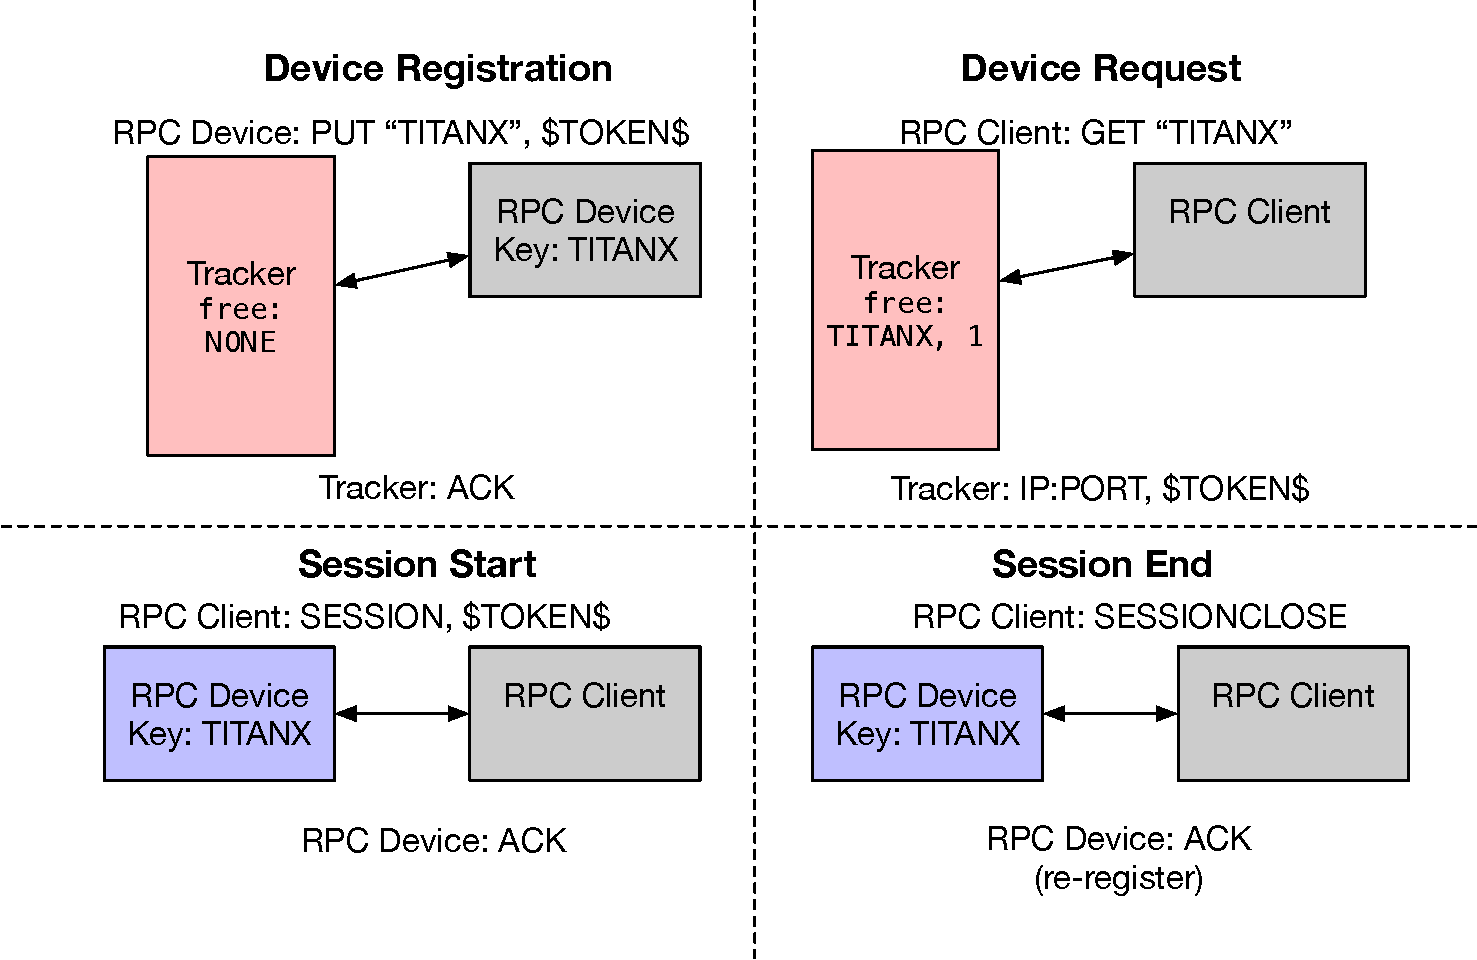
\includegraphics[width=\textwidth]{sys_diagrams/tracker.pdf}
\caption{Summary of the Control Plane (RPC Tracker) Protocol.
  1. An available device registers itself with the RPC tracker, providing a one-time use ``token`` value along with its device type~(in this case ``TITANX'').
  2. An RPC client requests a device of type ``TITANX.'' The tracker provides the address and one-time use token of an available device.
  3. The RPC client connects to the provided device and begins a session.
  4. The RPC client terminates its session; the RPC device registers itself as free to the tracker.
  Note that this logic is typically \emph{internal} to an optimization pipeline and transparent to the user seeking to change optimization algorithms.
}\label{fig:tracker}
\end{figure}
We provide a tracker~(i.e. resource manager) to coordinate the resources provided by a pool of devices.
\autoref{fig:tracker} shows a basic protocol of the resource registration.
In our setup, each RPC runtime registers itself with the tracker when it is available for performance measurement/profiling.
When a pipeline wishes to profile a configuration, it requests a free RPC session corresponding to its desired device type.
The tracker removes the requested device from the pool of free devices, and the devices re-registers itself with the tracker when profiling has been completed.
The pool of devices can be multiplexed across many developers or strategies for optimizing deep learning workloads on hardware.
%Multiplexing also naturally supports load balancing and high utilization of hardware resources: even if a single user is performing optimization, they may profile entire batches of candidate configurations at once to leverage additional parallelism.
Our tracker is inspired by the model used by the cluster management system such as
Mesos~\cite{Hindman:Mesos} and Kubernetes~\cite{Burns:2016:BOK:2930840.2890784}, with the additional challenge of providing a runtime environment that runs on heterogeneous embedded devices.

\paragraph{Data Plane}
The RPC data plane does not require each user to have an identical development environment---the RPC runtime simply runs the provided code.
This flexibility allows different search spaces as well as search strategies (e.g., cost model implementations, optimization algorithms) to share the same pool of devices seamlessly.
The data plane of the RPC runtime allows as much compilation to be performed on the client side (or before the RPC boundary) as possible.
This reduces the burden on devices that may be a poor fit for heavy-duty compilation (of the programs that they run), such as IoT devices or mobile phones.
%A side benefit is that the chances of a failure in a given device--client session affecting other clients is reduced.
The RPC runtime enables portability of optimization strategies and computational graph declarations across devices.
After developing an optimization strategy for a hardware device target (e.g., Raspberry Pi), a user can quickly evaluate the same optimization strategy on an NVIDIA GPU as both share the same RPC interface.
%For devices that share an underlying architecture but different operating system stacks (e.g., a Raspberry Pi and Android phone), only the device target must be changed.
%This ease-of-use is a substantial departure from needing to manually specify compilation toolflows for each hardware device; the user only needs to request a different hardware device type from the RPC tracker.

%\paragraph{Implementation Requirements}
%The RPC runtime defines a clear and lightweight set of requirements for enabling deep learning optimization on a hardware device.
%We demonstrate this with an Android app that supports the runtime and RPC protocol, enabling optimization of deep learning workloads on Android devices.


%\subsection{Flexible Data Plane Protocol}
%\begin{figure}[t!]
%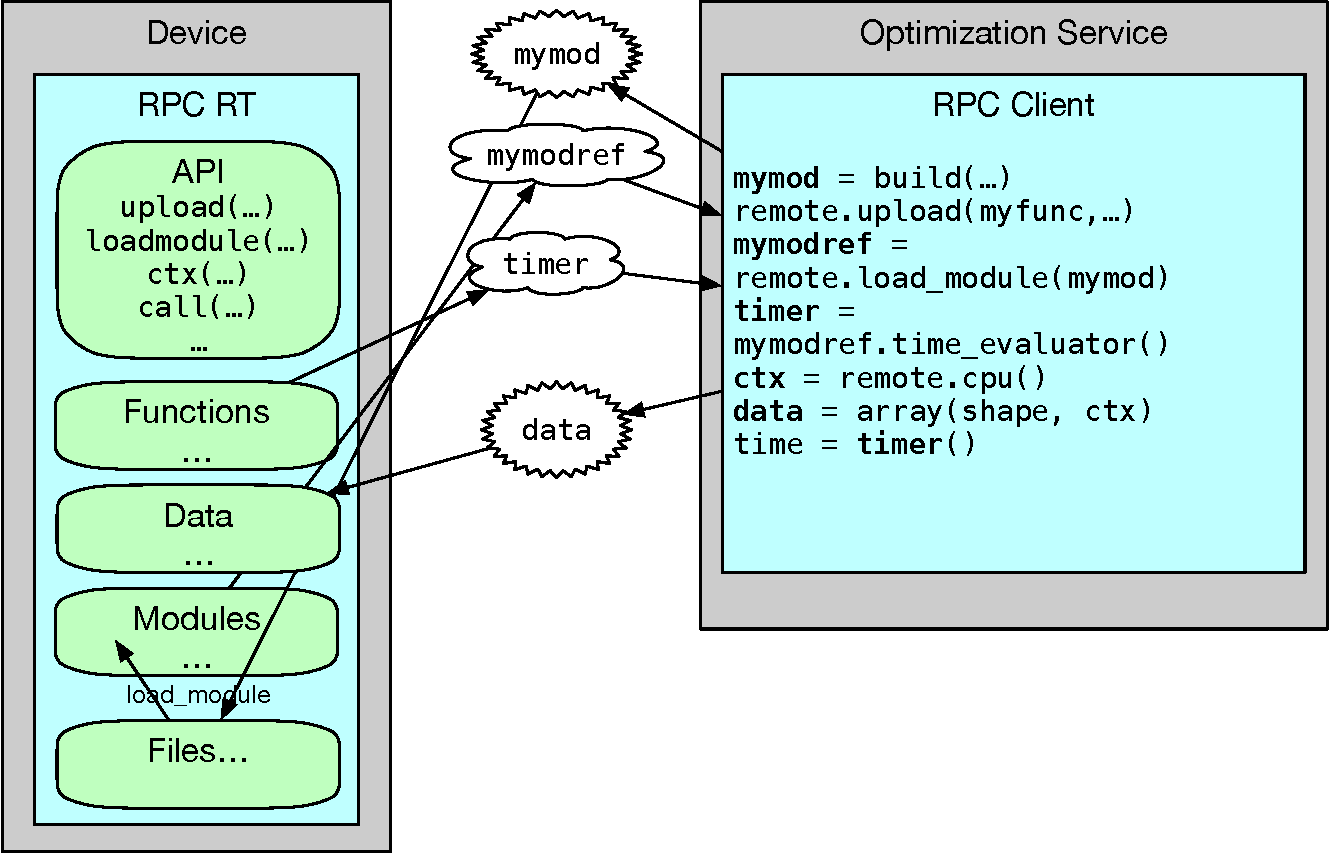
\includegraphics[width=0.5\textwidth]{diagrams/rpc.pdf}
%\caption{Summary of the RPC session protocol. A client builds a module corresponding to a proposed implementation of a workload.
%The compiled module is uploaded the RPC device and the client requests a handle to the loaded module.
%The client then requests a handle to a timer for evaluating the module, and passes input data to the timer to profile the execution of the proposed module.
%In an optimization scenario, this process is repeated many times for many proposed implementations.}
%\label{fig:protocol}
%\end{figure}
%One key difference from existing runtime systems is flexibility.
%Traditionally, the API between RPC clients and servers is slow-moving, with the implementations of function calls being fixed.
%In our setting, the goal of RPC is to implement a common interface for performance profiling on a wide range of hardware, where the implementations of each program are not fixed.
%To support this flexibility, we use RPC sessions that are stateful.
%As the RPC server typically does not know what implementation of an operator (the operator may even be unseen) it will execute during a session, the RPC client typically specifies the desired implementation over the course of a session.
%Using the RPC protocol, the client may change the implementations of various tensor programs on the RPC server (e.g., by uploading a dynamic library).
%The client may even take this to the extreme of modifying the RPC server's hardware, for example, by reprogramming the bitstream of an on-board FPGA.
%As shown in~\autoref{fig:protocol}, a typical application of RPC is to first cross-compile a proposed kernel implementation for a remote device, \emph{upload} the code to the remote device, and then profile the code on the remote device.


%We highlight a selection of the devices currently integrated with our system in \autoref{tbl:devices}.
% All devices marked with $\dagger$ have push-button automatic optimization support for a wide range of networks.

%\begin{table}[t]
%\begin{footnotesize}
%\begin{tabular} {l|c|c|c|c}
%Device &  \\
%\hline
%NVIDIA GPU&\checkmark\\
%AMD GPU&\checkmark\\
%ARM CPU&\checkmark\\
%ARM GPU&\checkmark\\
%x86 CPU&\checkmark\\
%ZYNQ FPGA&\checkmark\\
%\end{tabular}
%\end{footnotesize}
%\caption{Selection of devices currently supported and evaluated on our system.}
%\label{tbl:devices}
%\end{table}

\begin{table}[t]
\centering
\begin{tabular}{l|c|c|c}
\hline
HW&OK&Compile&Timeout/Misc.\\
\hline
gfx900 (AMD GPU)&61&143&84\\
rk3399 (ARM CPU)&55&86&147\\
pixel2 (ARM CPU)&89&86&113\\
\end{tabular}
\caption{Breakdown of failures tolerated when randomly traversing the search space of 9 VGG-16~\cite{simonyan2014very} workloads for various hardware targets.
32 configurations were sampled for each workload. Note that ``compile'' failures include configurations that violate constraints when checking against limits such as scratchpad size, available threads, etc.}\label{tbl:fault_tolerance}
\end{table}


\subsection{Fault Tolerance}

\begin{figure}[t!]
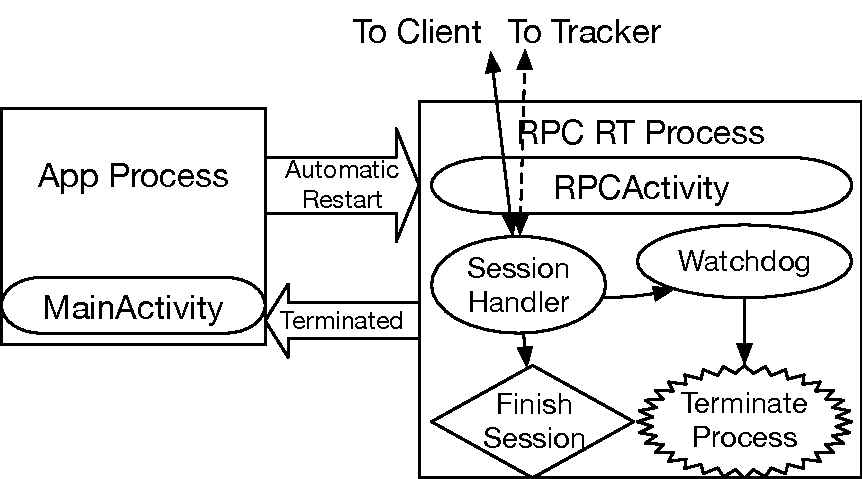
\includegraphics[width=\textwidth]{sys_diagrams/android.pdf}
\caption{Overview of the Android RPC runtime implementation.
  A second activity is dedicated to the RPC session in a separate process for fault tolerance, and also to ensure that the RPC session receives high OS priority by keeping its parent process on-screen. RPC session timeouts are enforced by a watchdog which ``races'' against the session processor.
  If the watchdog finishes first, the RPC process is terminated and restarted.}
\label{fig:android}
\end{figure}

At compile time, given the size of search spaces for each operator and hardware backend, each search space may contain many invalid configurations.
Invalid configurations may violate such restrictions such as scratchpad memory sizes on GPUs, maximum thread block/workgroup sizes in CUDA/OpenCL capable devices, or allocate more registers than the hardware supports.
 ~\autoref{tbl:fault_tolerance} shows an example of the distributions of failures encountered in practice.
%We provide several strategies for robustly handling faults both at compilation time (just after a given configuration in a search space is chosen) to run time, when a configuration has been deployed for measurement to a hardware device.
%We support compile-time checking of schedule configurations via checkers that inspect the maximum thread block/resource allocations required by each loop nest in the implementation, and comparing these values against those reported by CUDA/OpenCL.
At run time, each measurement forks a new workhorse process so that a buggy configuration that crashes the workhorse does not terminate the RPC server or prevent the device from re-registering with the RPC tracker.
Additionally, for devices with more exotic runtime environments, such as Android smartphones, we use an app with a separate watchdog~(shown in ~\autoref{fig:android}) process which restarts the workhorse RPC runtime if necessary.\footnote{We use this approach as the Android OS allocates CPU time depending on whether your process is responsible for the current on-screen Activity.}
%\TODO{cut many parts of this section, the user should not need to configure this directly}
%Internally, SeaNet supports several levels of \emph{timeout} functionality.
%Timing-out the measurement of a given schedule configuration may seem simple to implement, but in our experience it is a tricky task that requires careful consideration of the many sources of faults and potential race conditions (e.g., where a process succeeds after the timeout has been triggered but before it fires and terminates the request).
%Currently, the SeaNet environment uses timeouts for both \emph{compilation} and within the context of an RPC \emph{session}.
%This separation is important as it allows the time required to acquire an RPC device from the tracker to be factored out of a timeout.
%Otherwise, the timeout parameter is sensitive to the time spent waiting for an RPC device to become available, which is dependent on the utilization of the pool of RPC devices.
%Nevertheless, timeout remains important to ensure that optimization proceeds efficiently for a wide range of hardware devices, as poor schedule configurations can be quickly pruned if the timeout is exceeded.
Finally, at the control plane level, the tracker gracefully switches between devices if a device becomes faulty and fails to respond to incoming requests.
This property is essential in ensuring that a few faulty devices do not interfere with long running optimization tasks by polluting the measurement data.



%\section{Reference Datasets}
%To allow users to quickly bootstrap algorithms, we include several datasets collected on popular models and %hardware targets.
%This datasets kernel configurations that are competitive with state-of-the-art hand-rolled kernel %implementations specialized to each hardware platform.
%These datasets allow researchers to both quickly evaluate cost model prototypes (how accurately a cost 
%model can predict the performance of a kernel), peak-performance-model prototypes (how accurately a model %can predict the peak-performance of a kernel), and the  

\section{Baseline Implementations and Evaluation}
To highlight the flexibility of SeaNet across algorithms and hardware devices, we present descriptions of baseline implementations of SeaNet modules and evaluations of their performance starting with the first task, optimizing kernels for a given deep learning model.
We visualize the efficiency of different optimization pipelines by observing which pipeline achieves the best performance (of an evaluated program configuration) in the fewest \emph{trials} (measurements on hardware).
In our evaluation, we first seek to characterize two main types of optimization pipelines first: blackbox pipelines (e.g., evolutionary algorithms and random search), and cost-model driven baselines.
The pipelines evaluated on either a desktop GPU (NVIDIA 1080 Ti) or a Mobile CPU (ARM Cortex-A72) as denoted in their corresponding figure titles.
We then explore which sampling and model optimizing strategies are best given a particular cost model for the first task.
Following the first task, we visit the second task of predicting peak performance using different regression models.
\begin{figure}[tb]
\begin{center}
\begin{subfigure}[]{\textwidth}
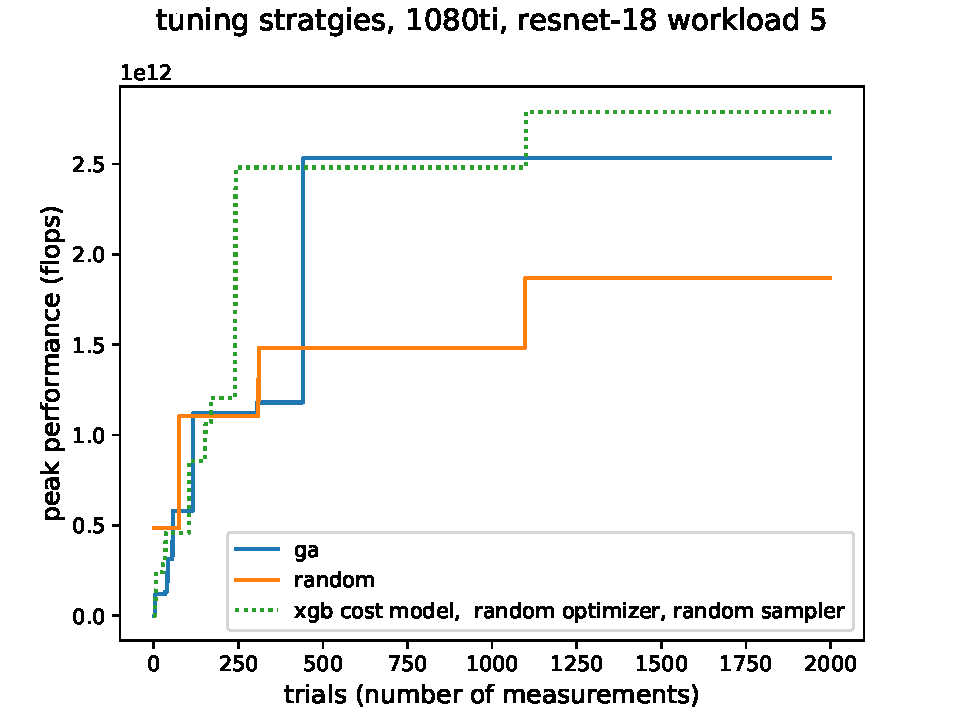
\includegraphics[width=\textwidth]{sys_figures/blackbox1080tiresnet-18_5_.pdf}
\end{subfigure}
\end{center}
\begin{center}
\begin{subfigure}[]{\textwidth}
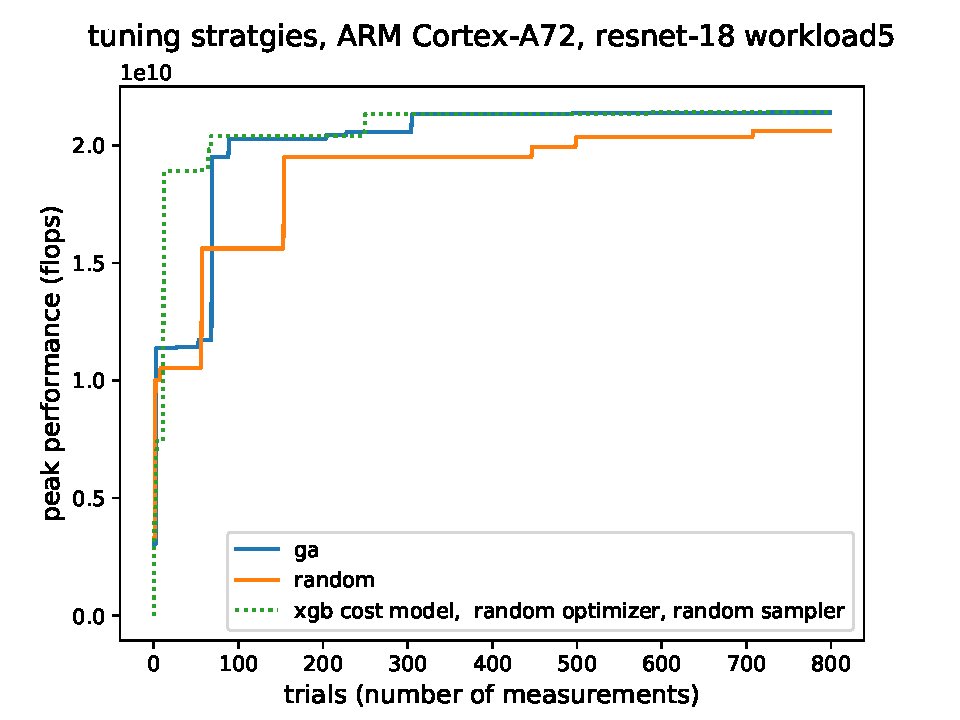
\includegraphics[width=\textwidth]{sys_figures/blackboxrk3399_resnet-18_5_.pdf}
\end{subfigure}
\end{center}
%\begin{subfigure}[]{\textwidth}
%\includegraphics[width=0.5\textwidth]{figures/blackbox%1080tiresnet-18_7_.pdf}
%\end{subfigure}
\caption{Task 1: Blackbox optimization pipelines compared with cost-model driven pipelines on a convolution kernel from ResNet-18~\cite{He_2016_CVPR}. Here, the XGBoost cost model is used to filter randomly proposed configurations that are then randomly sampled. The bottom plot shows an example of an ``easier'' optimization task, where all three approaches quickly achieve good performance.}
\label{fig:blackbox}
\end{figure}

\begin{figure}[tb]
\begin{center}
%\begin{subfigure}[]{\textwidth}
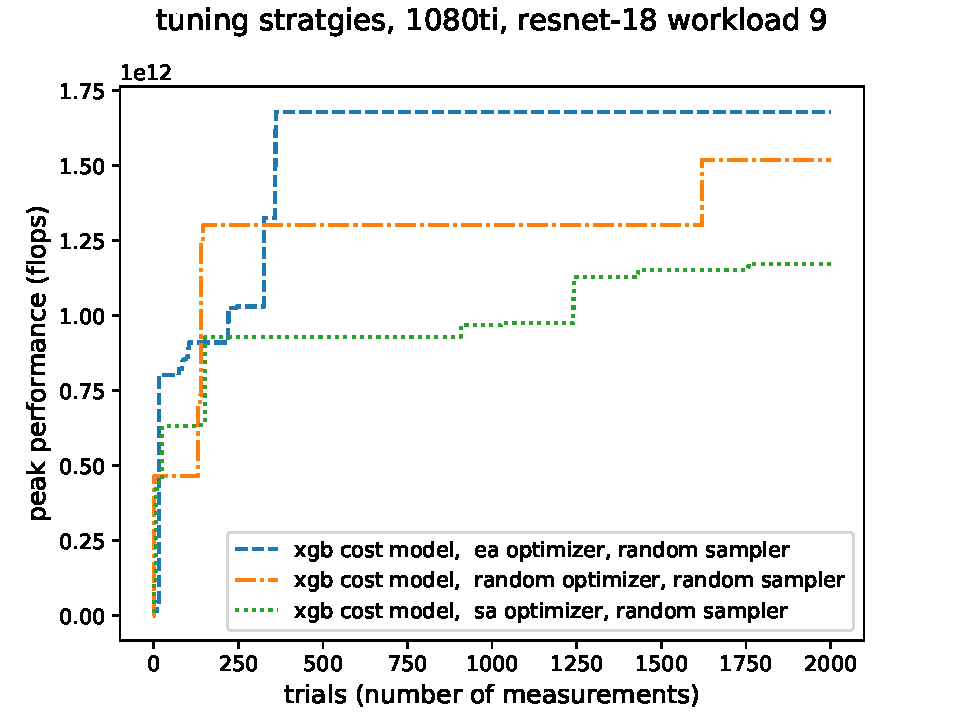
\includegraphics[width=\textwidth]{sys_figures/optimizer1080tiresnet-18_9_.pdf}
\end{center}
%\end{subfigure}
%\begin{subfigure}[]{\textwidth}
%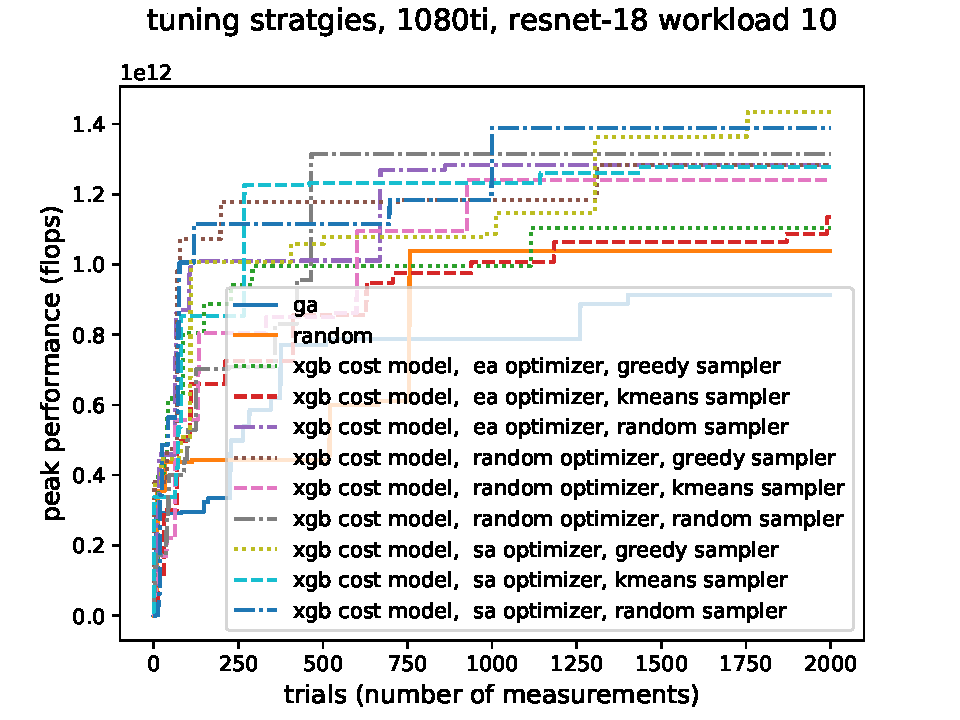
\includegraphics[width=0.4\textwidth]{figures/all1080tiresnet-18_10_.pdf}
%\end{subfigure}
\caption{Task 1: Comparison of model optimizers with random sampling. On many workloads, we find that the evolutionary algorithm works the best with random sampling.}
\label{fig:optimizers}
\end{figure}
\begin{figure}[tb]
\begin{center}
%\begin{subfigure}[]{\textwidth}
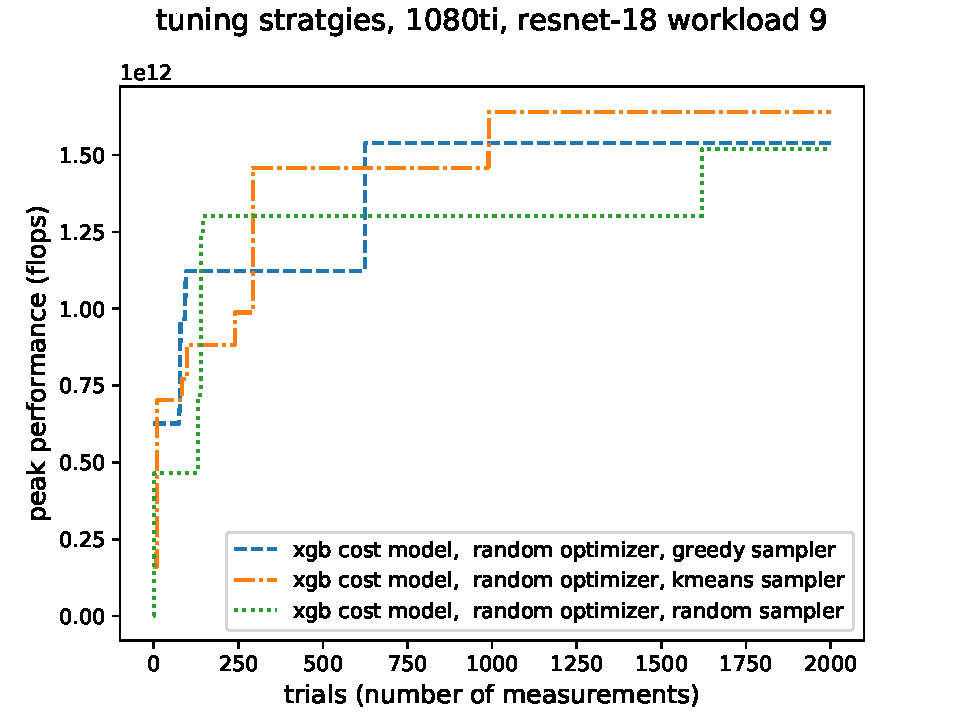
\includegraphics[width=\textwidth]{sys_figures/sampler1080tiresnet-18_9_.pdf}
%\end{subfigure}
%\begin{subfigure}[]{\textwidth}
%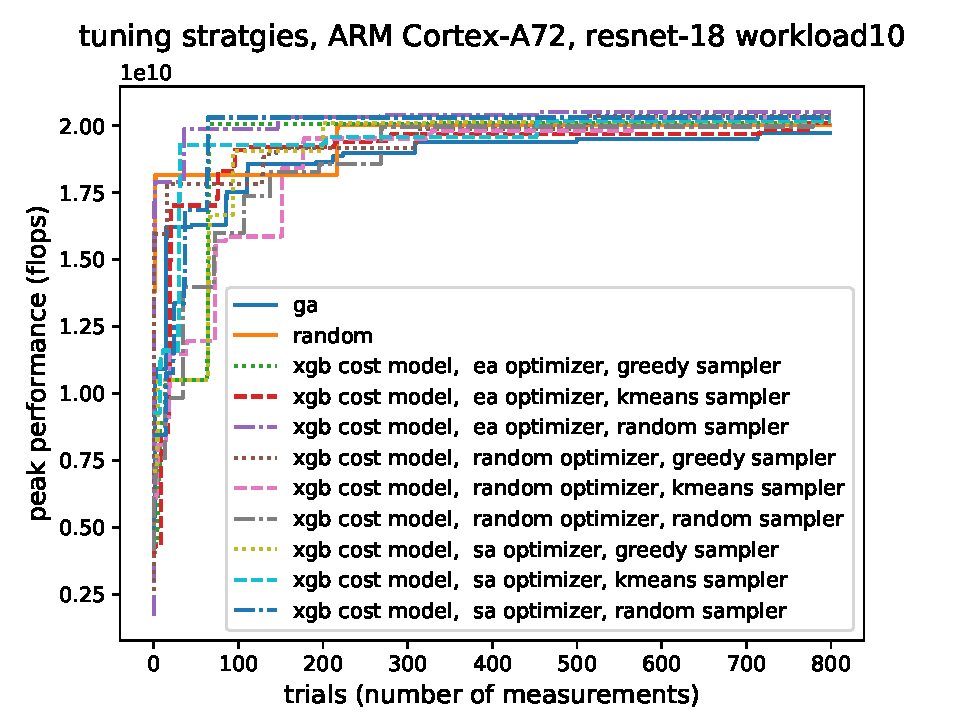
\includegraphics[width=0.4\textwidth]{figures/allrk3399_resnet-18_10_.pdf}
%\end{subfigure}
\caption{Task 1: Comparison of samplers with random proposals. On many workloads, we find that $k$-means sampling works the best with random proposals. Intuitively, this makes sense as K-Means sampling achieves the highest sample diversity.}
\label{fig:samplers}
\end{center}
\end{figure}

\begin{figure}[ht]
\begin{center}
%\begin{subfigure}[]{\textwidth}
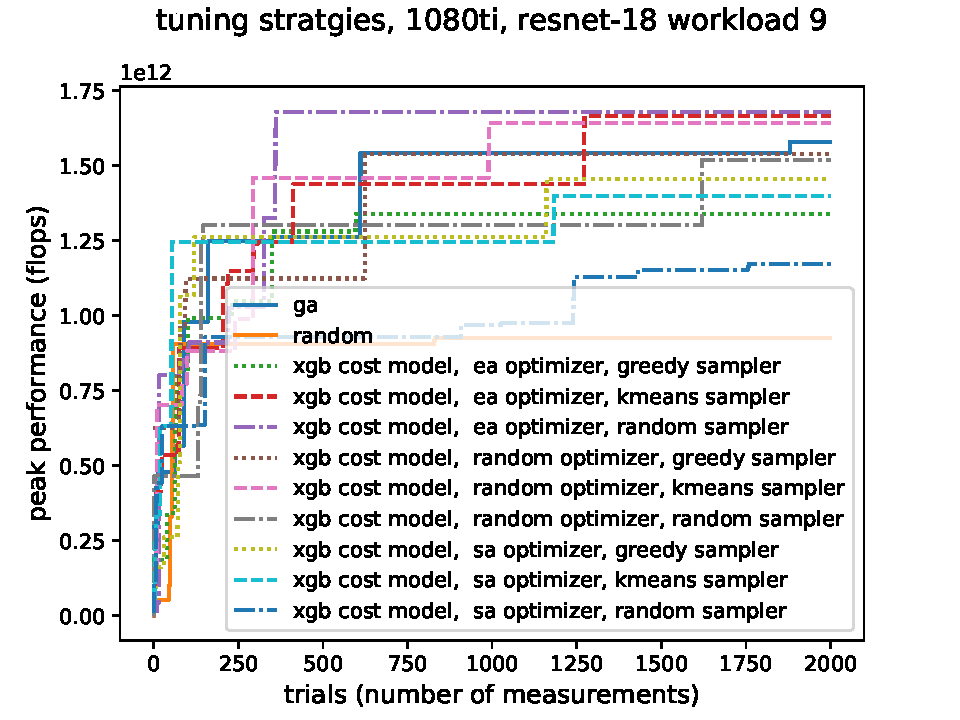
\includegraphics[width=\textwidth]{sys_figures/all1080tiresnet-18_9_.pdf}
\caption{Task 1: Comparison of all pipelines. All methods outperform the random baseline on this workload, with many of the best performing pipelines relying on an evolutionary algorithm (either as the optimizer or in blackbox form).}
\label{fig:all}
\end{center}
\end{figure}




\paragraph{Task 1: Optimization Pipeline Variants}
For the first task, we evaluate the efficiency of a variety of optimization pipelines.
At the highest level, these can be divided between \emph{blackbox} approaches that do not attempt to explicitly model the performance of different configurations in a search space, and \emph{cost-model} driven approaches that use a cost-model to estimate the performance of previously unseen configurations.
The cost model can any feature representation that can be derived from program configurations as input.
For simplicity, we base our features on the concrete values of the choices in each configuration space in this evaluation, though in practice more sophisticated approaches (e.g., using AST structures) are feasible.
We first compare the performance of two blackbox pipelines an genetic algorithm (GA) and random search with a cost-model driven pipeline that proposes many configurations randomly before filtering them through a cost model and then sampling among a promising subset of the proposed configurations randomly in ~\autoref{fig:blackbox}.
Here, we see that using a cost model can improve the efficiency of optimization (by using fewer hardware measurements) to reach the same level performance on more difficult workloads, yet all three methods remain comparable on easier workloads.
Next, we seek to characterize the difference between cost-model pipelines that use a model optimizer to propose promising configurations.
In this setting, we introduce a simulated annealing (SA) model optimizer and an evolutionary algorithm model optimizer (EA) alongside the random model optimizer.
We refer to the optimizer as EA while it is logically identical to the blackbox GA, with the difference being that the fitness scores of the GA are obtained through actual hardware measurement (blackbox), whereas the EA queries a cost model for fitness scores.
In this comparison (~\autoref{fig:optimizers}), we see that the evolutionary algorithm performs best with random sampling on many of the challenging workloads.
Interestingly, for the workload shown, the SA optimizer is the worst, though for many other workloads it is competitive with the EA optimizer.
We suspect that in many cases, the optimizers require hyperparameter tuning for ideal efficiency.

We then seek to characterize the differences in the remaining component of the optimization pipeline: the sampler.
Here, we provide a $k$-means and greedy sampler alongside the random sampler which chooses configurations filtered by the cost model randomly.
The $k$-means sampler first clusters points proposed by the model optimizer with $k$ set to the number of measurements to be performed, whereas the greedy sampler simply picks the top-$k$ highest scoring proposals.
Here, we find that the $k$-means sampler tends to do well on workloads where exploring a diverse set of configurations in the search space is beneficial.
Finally, we show an example of all pipelines evaluated so far in ~\autoref{fig:all}.
While the relative efficiency of different pipelines can be tricky to interpret, we see that all pipelines surpass random search, and that evolutionary strategies (including blackbox versions) do well.

%This cost model can take in discrete knob values (e.g., the choice of each tuning parameter) as input or lower-level information from the program AST for more advanced users.
%Additionally, in our evaluation, we show linear regression and MLP baselines that are easy-to-implement wrappers around scikit-learn libraries.
%\subsection{Example: End to End Simulated Annealing Pipeline}
%We present an example end-to-end optimization pipeline that populates each of the individual optimization components with empirically validated choices.
%This example optimizer uses simulated annealing-driven configuration proposal, guided by a gradient-boosted tree cost model, with $\epsilon$-greedy sampling.
%At a high level, this example is a straightfoward implementation


%A random model optimizer simply proposes random points in the search space and returns some top-$k$ as estimated by the cost model.
%A random sampler simply chooses random points in the proposed set to evaluate.
%~\autoref{fig:optimizers} compares different model optimizers with random sampling, and ~\autoref{fig:samplers} compares different samplers with random proposals.

%Overall, the effectiveness of each solution seems to be workload dependent.
%We can see in ~\autoref{fig:blackbox} the cost-model driven strategy is competitive in all three scenarios, yet does best when there is a challenging workload that requires many trials to reach peak performance.
%On some tasks, the genetic baseline is competitive, and on the workloads requiring the fewest trials to tune the random baseline is competitive.
%When proposing configurations randomly, we find that the K-Means sampler performs well as it intuitively enforces the most diversity among samples---ensuring that no samples are wasted to similar configurations.
%\TODO{do we want to do greedy sampling when comparing different proposers?}
%When sampling randomly, we find that the evolutionary optimizer tends to propose the best configurations for many workloads.



\paragraph{Task 2: Peak Performance Prediction}
\begin{figure}[ht]
\begin{center}
 \begin{subfigure}[]{\textwidth}
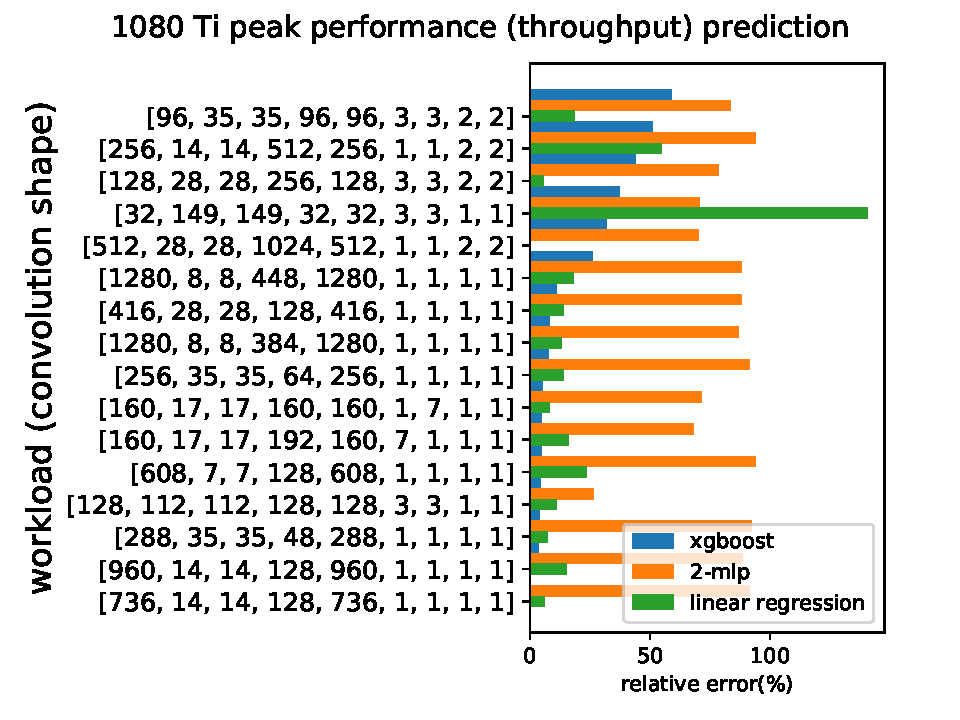
\includegraphics[width=\textwidth]{sys_figures/cuda_1080ti_binary_throughput.pdf}
%\caption{Predicted vs. actual peak-performance on a gradient boosted model trained on pretuned workloads for the 1080Ti.
%The vertical axis denotes shape parameters of 2D convolution
%Sorted from highest error to lowest. Orange bars show actual measure performance.}
\label{fig:peak1080ti}
\end{subfigure}
\end{center}
\begin{center}
 \begin{subfigure}[]{\textwidth}
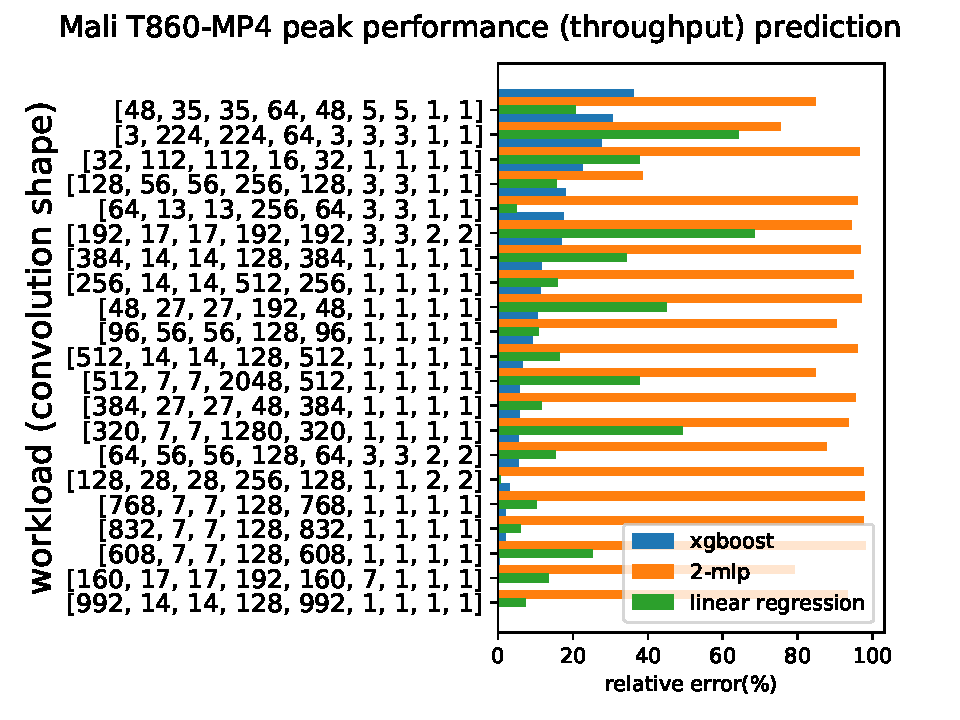
\includegraphics[width=\textwidth]{sys_figures/mali_rk3399_binary_throughput.pdf}
%\caption{Predicted vs. actual peak-performance on a gradient boosted tree model trained on pretuned workloads for the Mali T860-MP4. 
%The vertical axis denotes shape parameters of 2D convolution.
%Sorted from highest error to lowest. Orange bars show actual measure performance.}
\label{fig:peakmali}
\end{subfigure}
\end{center}
\end{figure}
\begin{figure}[ht]
\ContinuedFloat
\begin{center}
\begin{subfigure}[]{\textwidth}
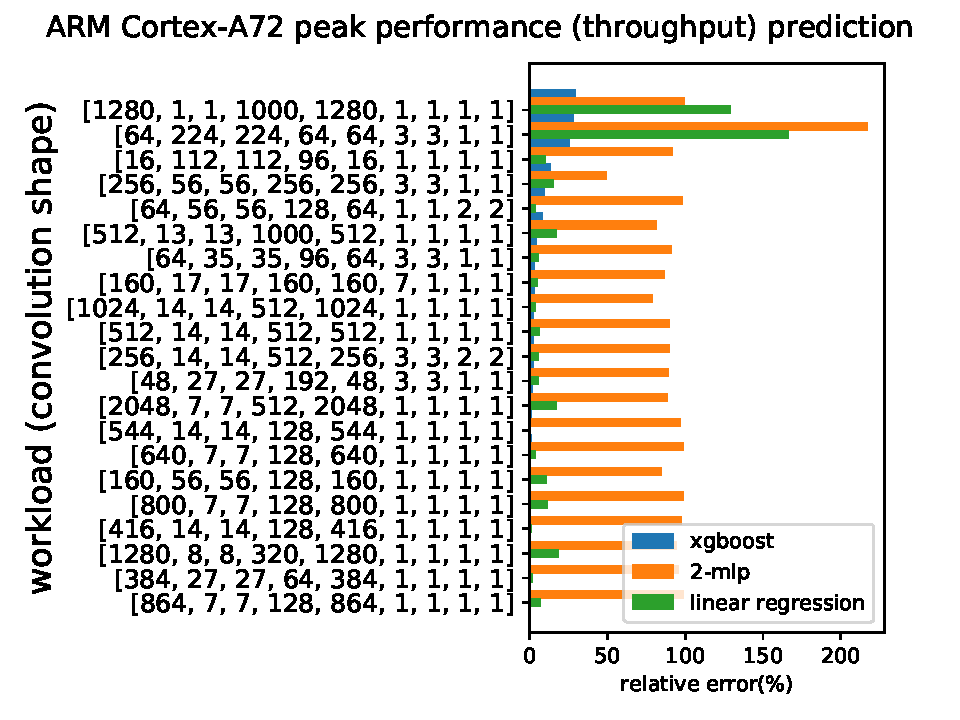
\includegraphics[width=\textwidth]{sys_figures/arm_cpu_rk3399_binary_throughput.pdf}
\label{fig:peaka72}
\end{subfigure}
\end{center}
\caption{Task 2: Relative error of predicted vs. actual peak-performance with various regression models trained on pretuned workloads for the NVIDIA 1080Ti, Mali T860-MP4, and ARM Cortex-A72.
The vertical axis denotes shape parameters of 2D convolution.
Workloads are sorted from highest error to lowest. Orange bars show actual measured performance.}
\label{fig:peak}
\end{figure}
Moving to the second task, we seek to characterize the effectiveness of different typical regression models for predicting peak performance. 
We train a type of model on a subset of pretuned-operator performance data and use it to predict performance on the held-out set.
~\autoref{fig:peak} shows these results, compared with linear regression and MLP baselines.
With minimal data preprocessing (converting dataset features to one-hot encodings), we find that peak-performance on a gradient tree boosting model yields promising results.
We expect that peak performance prediction can be integrated with performance driven NAS approaches that include with program optimization in the NAS search loop.

\section{Conclusion}
Automatic machine learning program optimization is becoming a fruitful area of research for both machine learning algorithms and downstream optimization tasks such as NAS and graph optimization.
However, one major impediment to researchers currently working in the field is the lack of a reusable system stack spanning predefined search spaces to device-specific code generation and transparent runtimes for benchmarking implementations and prototyping optimization pipelines.
In this paper, we presented SeaNet, which aims to fill this gap by enabling machine learning researchers to plug in their custom optimization algorithms into challenging optimization tasks.
We presented two typical problem settings: the optimization of a collection of kernels corresponding to deep learning workloads, and peak-performance prediction for previously unseen kernels.
Additionally, we give a detailed description of a device-portable RPC system that enables users to quickly move between different hardware devices without affecting their algorithm implementation.
Finally, we presented evaluations of modular implementations for the tasks on various hardware devices to highlight the flexibility of the SeaNet environment.

%In future work, we hope to advance the performance of the baselines further and integrate downstream tasks such as neural architecture search and graph optimizations.
%Reusable environments for research and exploration are essential building blocks at all levels of the system stack, just as benchmarks have paved the way for much of the progress achieved in deep learning today.
% Note use of \abovespace and \belowspace to get reasonable spacing
% above and below tabular lines.


% Acknowledgements should only appear in the accepted version.
%\section*{Acknowledgements}
%
%\textbf{Do not} include acknowledgements in the initial version of
%the paper submitted for blind review.
%
%If a paper is accepted, the final camera-ready version can (and
%probably should) include acknowledgements. In this case, please
%place such acknowledgements in an unnumbered section at the
%end of the paper. Typically, this will include thanks to reviewers
%who gave useful comments, to colleagues who contributed to the ideas,
%and to funding agencies and corporate sponsors that provided financial
%support.
%
%
%% In the unusual situation where you want a paper to appear in the
%% references without citing it in the main text, use \nocite
%\nocite{langley00}

%\clearpage
%\bibliography{paper}
%\bibliographystyle{sysml2019}
%%
%
%%%%%%%%%%%%%%%%%%%%%%%%%%%%%%%%%%%%%%%%%%%%%%%%%%%%%%%%%%%%%%%%%%%%%%%%%%%%%%%%
%%%%%%%%%%%%%%%%%%%%%%%%%%%%%%%%%%%%%%%%%%%%%%%%%%%%%%%%%%%%%%%%%%%%%%%%%%%%%%%%
%% SUPPLEMENTAL CONTENT AS APPENDIX AFTER REFERENCES
%%%%%%%%%%%%%%%%%%%%%%%%%%%%%%%%%%%%%%%%%%%%%%%%%%%%%%%%%%%%%%%%%%%%%%%%%%%%%%%%
%%%%%%%%%%%%%%%%%%%%%%%%%%%%%%%%%%%%%%%%%%%%%%%%%%%%%%%%%%%%%%%%%%%%%%%%%%%%%%%%
%%\appendix
%%\section{Please add supplemental material as appendix here}
%%%
%%Put anything that you might normally include after the references as an appendix here, {\it not in a separate supplementary file}. Upload your final camera-ready as a single pdf, including all appendices.
%%
%%%%%%%%%%%%%%%%%%%%%%%%%%%%%%%%%%%%%%%%%%%%%%%%%%%%%%%%%%%%%%%%%%%%%%%%%%%%%%%%%
%%%%%%%%%%%%%%%%%%%%%%%%%%%%%%%%%%%%%%%%%%%%%%%%%%%%%%%%%%%%%%%%%%%%%%%%%%%%%%%%
%
%
%\end{document}


% This document was modified from the file originally made available by
% Pat Langley and Andrea Danyluk for ICML-2K. This version was created
% by Iain Murray in 2018. It was modified from a version from Dan Roy in
% 2017, which was based on a version from Lise Getoor and Tobias
% Scheffer, which was slightly modified from the 2010 version by
% Thorsten Joachims & Johannes Fuernkranz, slightly modified from the
% 2009 version by Kiri Wagstaff and Sam Roweis's 2008 version, which is
% slightly modified from Prasad Tadepalli's 2007 version which is a
% lightly changed version of the previous year's version by Andrew
% Moore, which was in turn edited from those of Kristian Kersting and
% Codrina Lauth. Alex Smola contributed to the algorithmic style files.
